\section{Results}
\subsection{Bayesian Model}



\begin{figure}
	\centering
	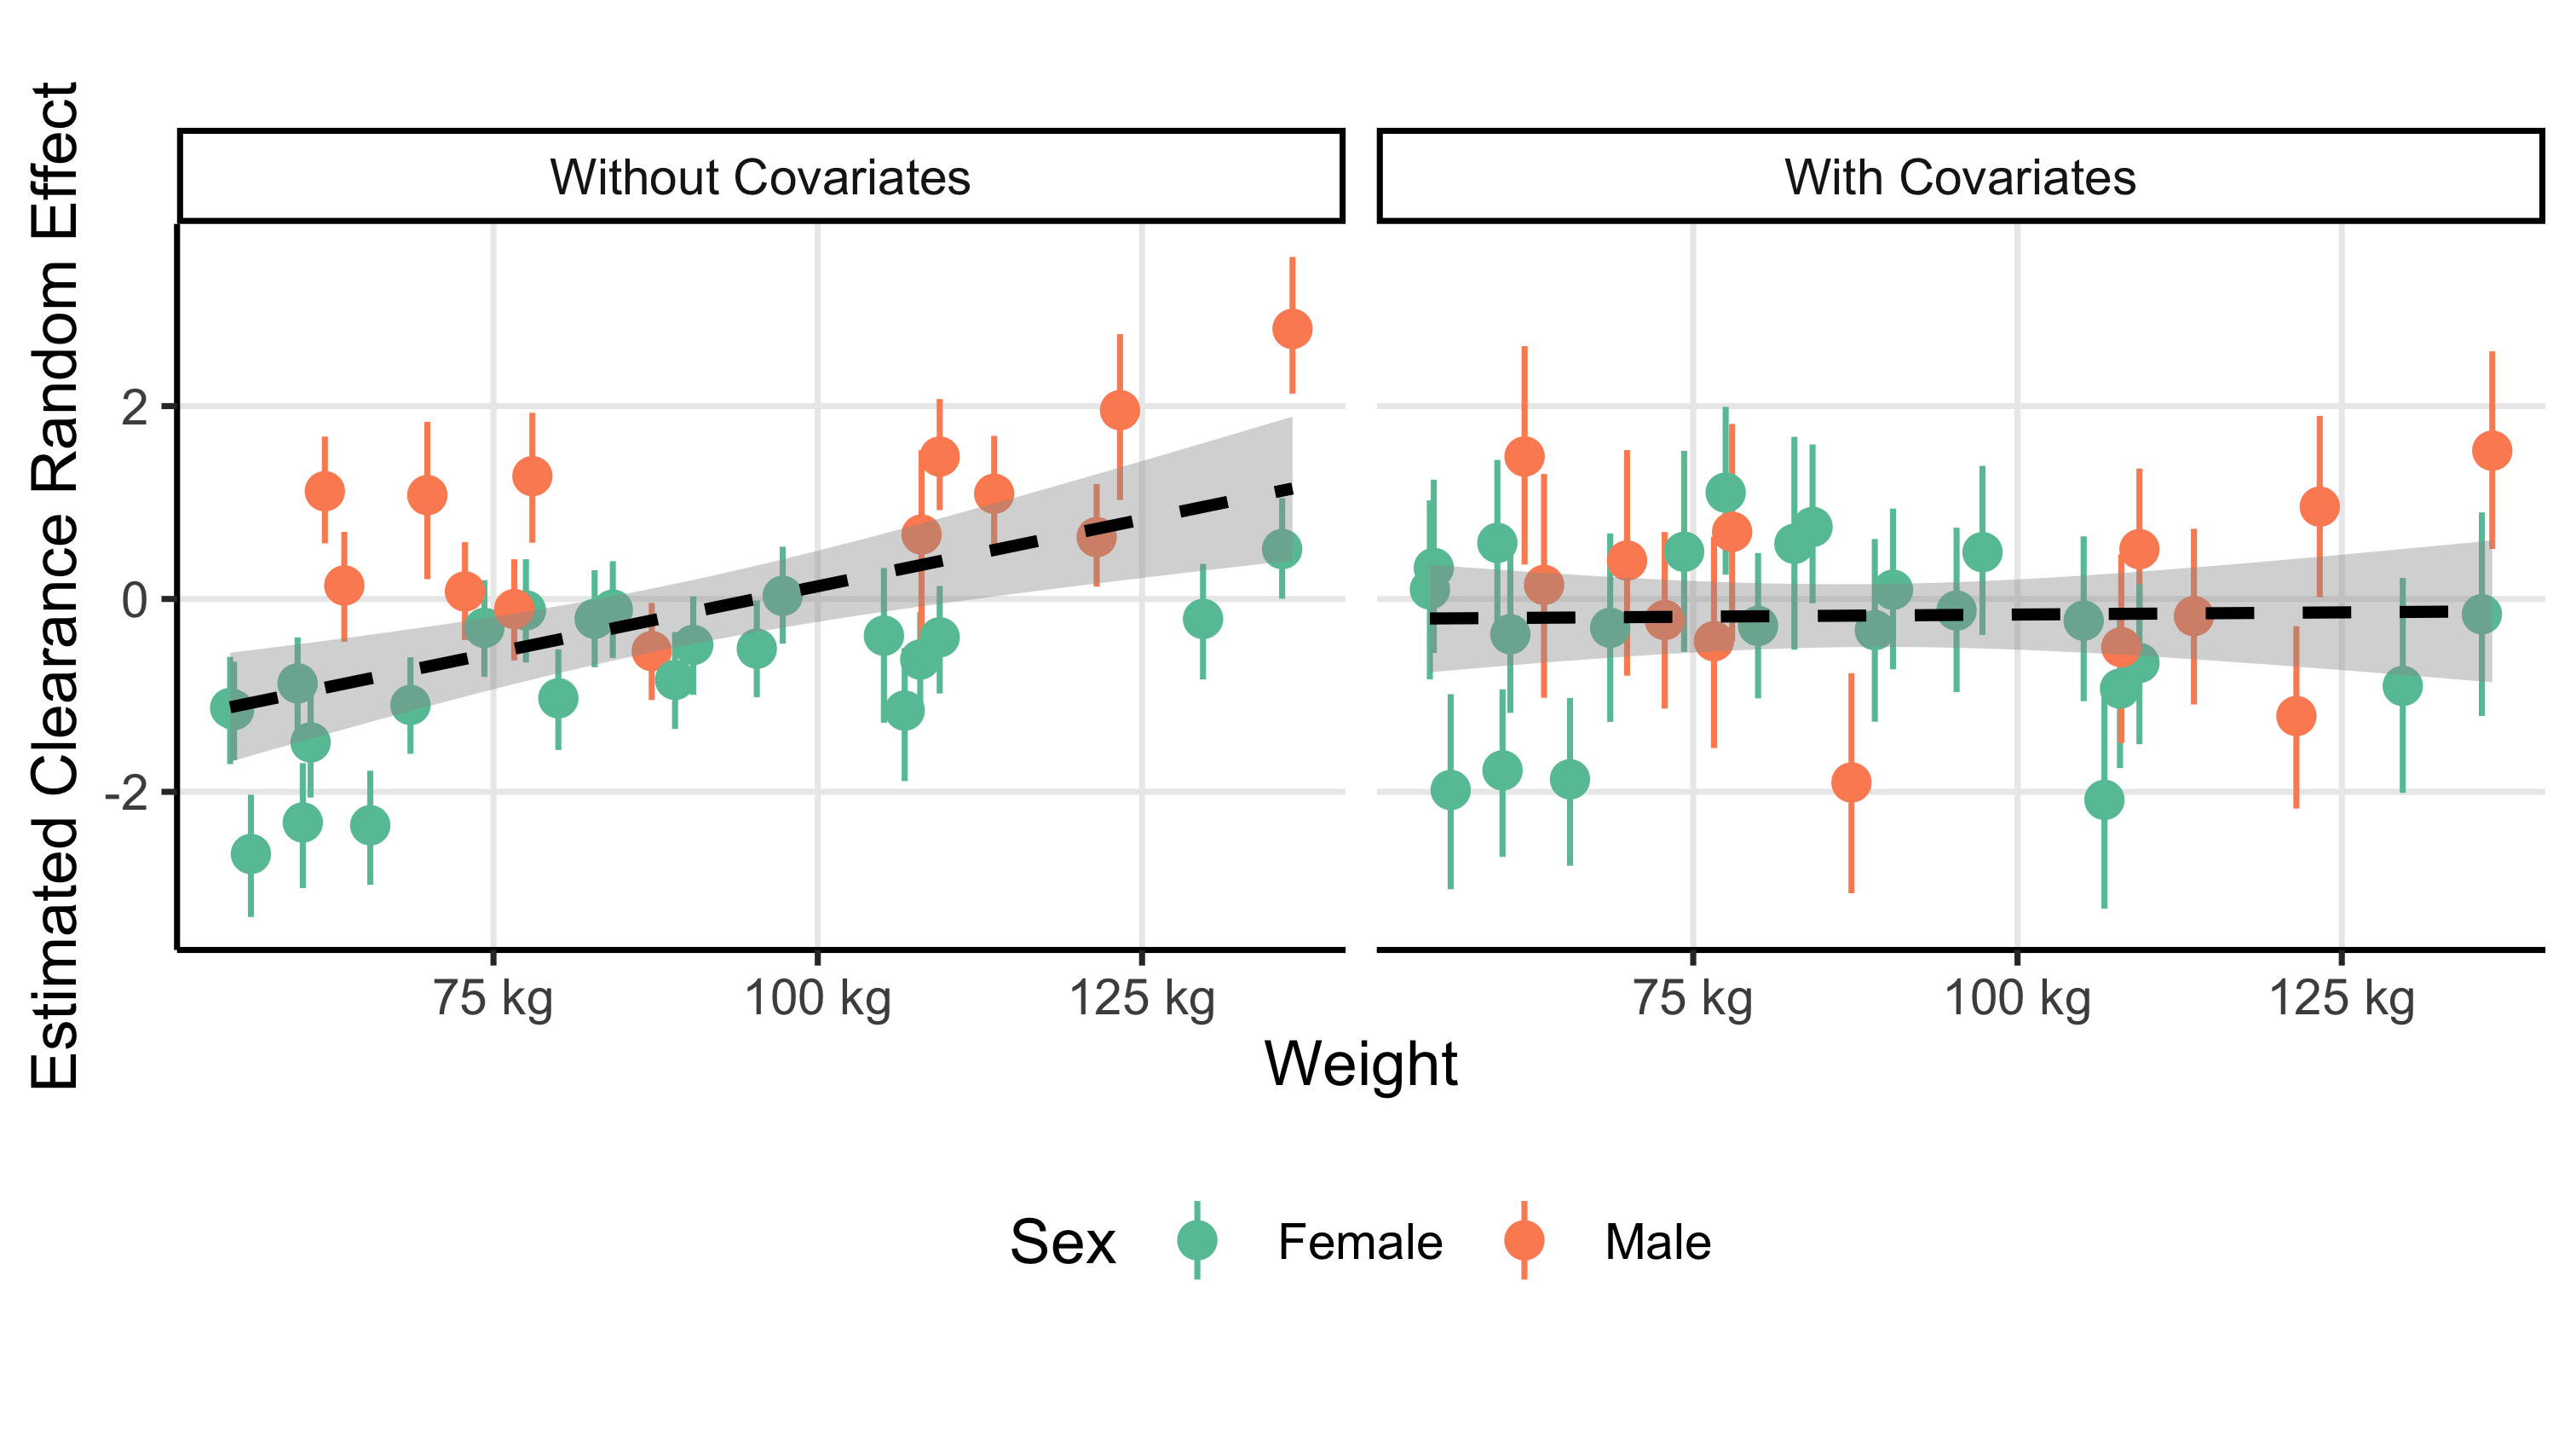
\includegraphics[width=\linewidth]{"figures/random_effects_change.png"}
	\caption{Random effects estimates for clearence rate $ Cl_i $and 95\% credible intervals (left).  Random effects estimates are colored by patient sex.  Prior to adjusting for covariates, a general trend in weight can be seen in the random effects.  Subjects who are heavier tend to have larger random effect, and males tend to have larger random effects than females of the same weight.  Patterns isuch as these indicate that weight and sex can be used to explain variation in the random effects.  After adjusting for sex and weight (right), the random effects have no discernable pattern.}
	\label{fig:randomeffectschange}
\end{figure}

In this section we present results of two different analyses.  We first assess the fit of our Bayesian model, as the model is crucial for our decision making experiments.  We then present the results of our decision making experiments.

We fit M1 to real pharmacokinetic data using Stan.  Stan monitors several markov chain diagnostics none of which detected problematic markov chain behavior, which indicates that Stan’s sampling algorithm was able to converge to the target distribution (0 divergences, all all Gelman-Rubin diagnostics<1.01, all effective sample size ratios  > 22\%).  

The inclusion of covariates in the model results in a better fit than excluding them. Shown in \cref{fig:randomeffectschange} are the estimated random effects for the clearance pharmacokinetic parameter of each subject as a function of weight.  Subject sex is indicated by color, the overall trend is shown in the black dashed line.  Failing to include subject sex and weight results in males having on average a larger random effect than females of the same weight, and heavier subejcts having a larger random effect than lighter subjects.  When covariates are added into the model, the variation in the random effects attenuates, resulting in closer alignment to model assumptions. A better fit to the data means data generate from the model may be closer aligned with the true data generating process.

Examining the posterior distributions of the regression coefficients provides further insight.  Subject weight increases the expected value of alpha (which is used to compute the elimination and absorption rates in the first order one compartment PK model.  The parameter $ \alpha $ is the ratio of how fast the drug exists the central compartment to how fast the drug enters the central compartment) as well as the time to max concentration.  There appears to be an effect of sex on $ \alpha $ (males have smaller alpha than females, meaning the drug leaves their central compartment slower or enters the central compartment quicker), however the uncertainty is large (estimated effect -0.2 on the logit scale, 95\% credible interval -0.54 to 0.15). See supplementary table X for a full summary of the regression coefficients.


\begin{figure}
	\centering
	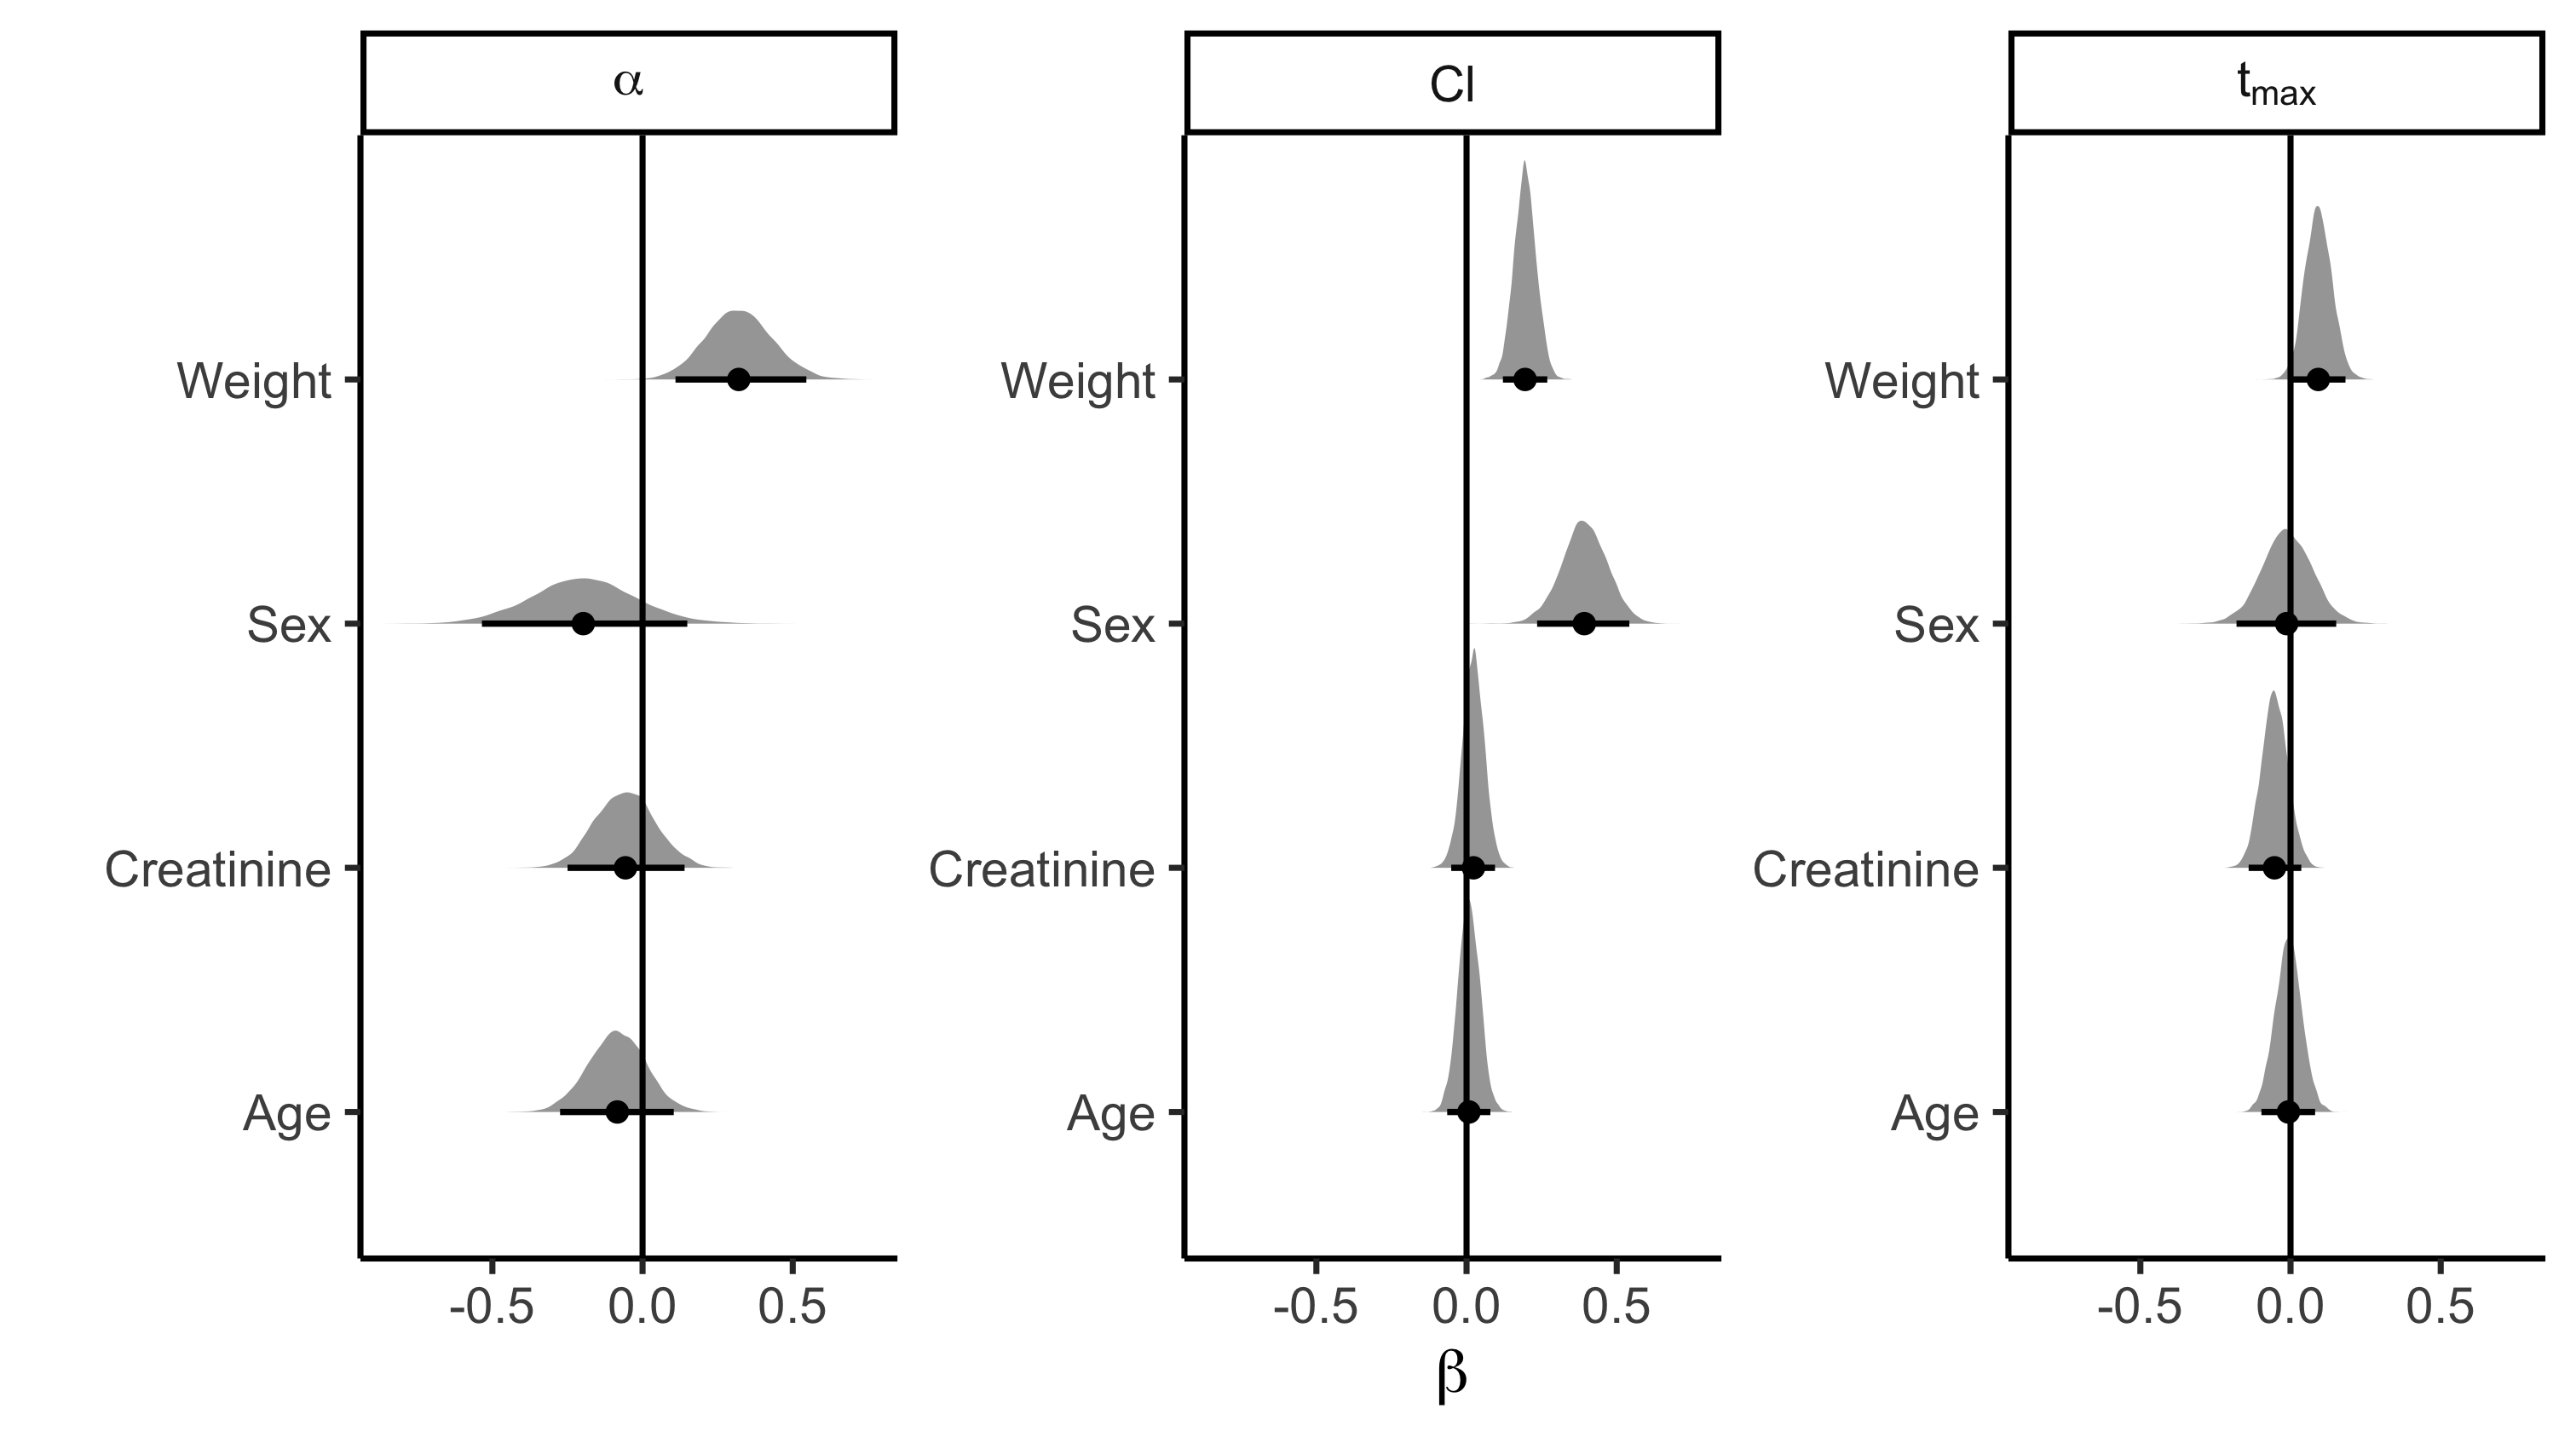
\includegraphics[width=1\linewidth]{figures/coef_vals}
	\caption{Posterior distributions of regression coefficients. Expectations are shown as black dots, 95\% credible intervals are shown as horizontal black lines.  Solid black vertical line is $\beta=0$ for reference.  Note, regression coefficients for $Cl$ and $t_{max}$ act multiplicatively (a one unit increase in weight leads to a change in $Cl$ of $\exp(\beta)$), while regression coefficients for $\alpha$ are interpreted on the log odds scale.}
	\label{fig:coefvals}
\end{figure}


Model training error sees a very small improvement.  Including subject covariates decreases model training error from 6.89 ng/ml to 6.84 ng/ml. Estimates of concentration uncertainty remain similar between the two models as well.  We conclude the inclusion of covariates in the model improves model inferences but does not improve the fit of the model to the data in any substantial way.  Either model would require additional validation prior to using in a predictive capacity.

\subsection{Simulation Results}

We consider 6 modes of personalization which range in the amount of information used in the decision process as well as burden placed on the patient and clinic, and burden of implementation.  We present the results of our simulation in figure X below in terms of difference between theoretically largest reward and reward achieved by the mode of personalization.  The results are ordered from least amount of information and burden (top) to most amount of information and burden (bottom).

Modes of personalization which use less information have a larger difference (i.e. yield smaller reward on average than what is theoretically possible).  The no covariate model (which uses no information about the subject) performs worst with a median difference of 0.19.  The distribution of differences for this mode is right skewed with some differences exceeding 0.95, meaning the subject could have been in range for nearly the entire time but the mode selected a dose which failed to put the subject in range. 

The use of covariates in the model nearly cuts the difference in half, achieving an average difference of 0.1 with smaller right skew.  There is a diminishing in the difference in rewards as additional burden is undertaken. Modes which use observed concentration information (Covariate Model + 1 Sample, Optimal Sampling Time, and Q Learning) lead to marginally more reward on average.


\begin{figure}
	\centering
	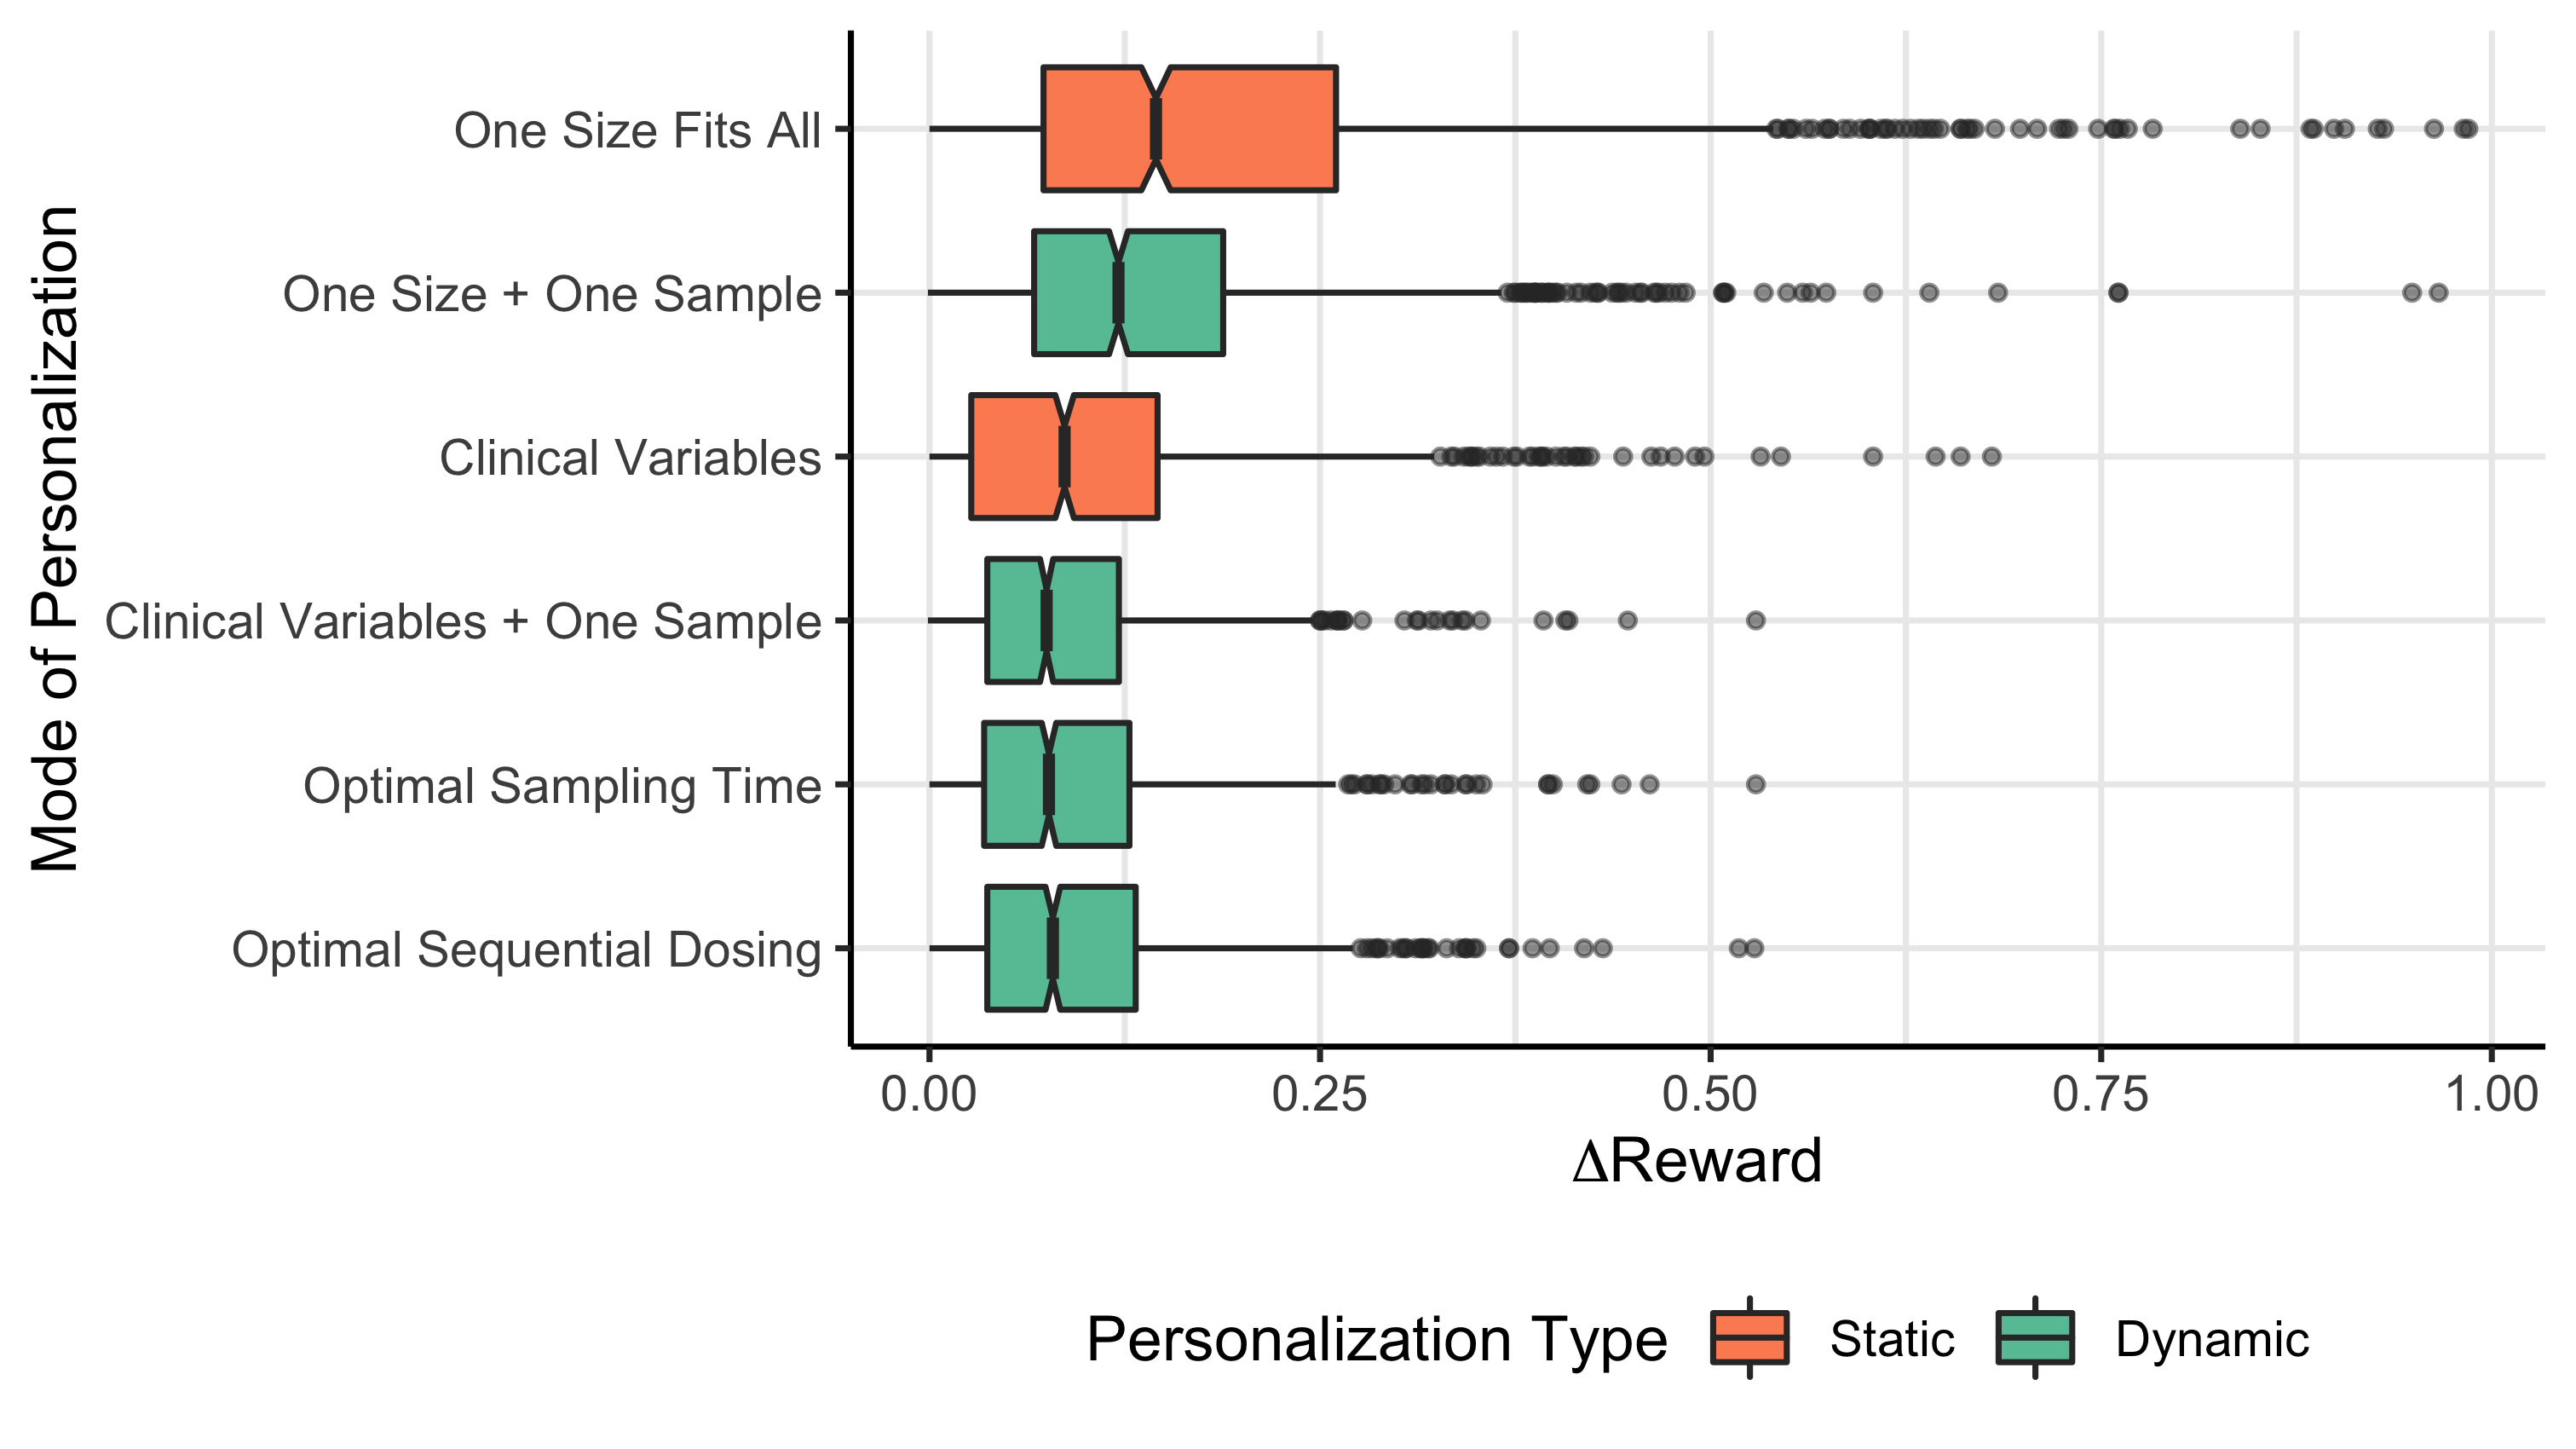
\includegraphics[width=1\linewidth]{figures/models_of_personalization_differences}
	\caption{Boxplots of the difference between theoretically largest reward and achieved reward for each of the 1000 simulated subjects. Subjects who achieve a reward close to their maximium reward have a difference on 0, subjects who achieve a reward less than their maximum have larger differences, with the largest difference being 1.}
	\label{fig:modelsofpersonalizationdifferences}
\end{figure}
